\documentclass[main.tex]{subfiles}
\begin{document}

\chapter{Evaluation}
In this chapter, the previously selected algorithms are uniformly compared. We present the results.
\section{Protocol}

This work aims to determine which plane detection algorithm is the most suitable for an AR/VR system. For this decision, we uniformly compare the algorithms selected in
Chapter~\ref{chap:Concept}. We split the comparison into two experiments conducted on different datasets: the 2D-3D-S and the
self-created FIN dataset. Since both datasets are fundamentally different, we will perform the experiments and the analysis separately and then compare the results.
First, we present the metrics used for comparison, followed by an outline of the used configurations of parameters for each experiment.

\subsection{Metrics}
\label{subsec:metrics}
\paragraph{Accuracy}
To quantify the accuracy of the plane detection algorithms, we use the detected planes and the created ground truth to calculate the three following
metrics: Precision, Recall, and the F1-score. The procedure of calculation is taken from~\cite[Section~4]{Araújo_Oliveira_2020} and detailed
in Section~\ref{sec:metrics}.


\textcolor{red}{hier noch mehr ins detail gehen? (antwort) \underline{\hspace{2cm}}}

\paragraph{Time Measurements}
\label{par:time}
In addition to the accuracy, we are interested in the real-time applicability of an algorithm. We present two definitions
of \textit{real-time} in Section~\ref{sec:realtime}.
Since we have two definitions of real-time, it is helpful to introduce two metrics of computation times.
We divide the calculation into pre-processing, plane calculation, and post-processing.
The respective calculation times are in the following, referred to as $t_{pre}, t_{calc}$, and $t_{post}$.
This separation allows for an in-depth analysis. Furthermore, it allows us to determine
whether an algorithm is $RT_{calc}$. To determine whether an algorithm is $RT_{tot}$, we consider the
total computation time $t_{tot}$, which is the sum of the individual times:

\begin{equation}
    t_{tot} = t_{pre} + t_{calc} + t_{post}
\end{equation}

\textbf{\textcolor{red}{this still seems poorly placed}}
When recording a real environment, the point clouds grow incrementally over time.
Therefore, the average calculation times alone are of limited significance, as we expect shorter times for the start of a recording
and longer times for the most recent. Therefore, we consider the relationship between the point cloud size and the calculation time in
addition to average values. However, we do not evaluate the accuracy over time since as accuracy of an algorithm should be
independent of the size of the point cloud.


\textbf{\textcolor{red}{das hier eher in den BG oder?}}
RSPD, 3D-KHT and OBRG construct an octree during their pre-processing phase. Additionally, RSPD and OBRG perform an initial
estimation of normals. OPS estimates the normal vectors for a randomly chosen sample set of points.
During post-processing, OPS merges smaller planes if they pass a coplanarity test and then re-estimates the normals of the
resulting plane. In the post-processing step, OBRG refines the borders of detected planes by inserting
previously unallocated regions. RSPD and 3D-KHT do not perform post-processing.
The pre-and post-processing steps are summarized in Table~\ref{tab:pre-post}.


\begin{table}[H]
    \centering
    \begin{tabular}{c|cccc}
             & RSPD & OPS   & 3D-KHT & OBRG       \\ \hline
        Pre  & NE   & NE    & OC     & OC + NE    \\
        Post & /    & Merge & /      & Refinement
    \end{tabular}
    \caption{Pre-processing and post-processing steps of the plane detection algorithms. RSPD and 3D-KHT do not have any post-processing steps.}
    \label{tab:pre-post}
\end{table}

\subsection{Parameterization of Algorithms}
Because the datasets inherit different amounts of noise, it is necessary to modify the algorithms accordingly.
We thereby modify the algorithms' parameterization to achieve more noise robustness.
In the following, the parameterizations of the algorithms with respect to the two experiments are outlined.
Therein, we refer to the parameterization of the 2D-3D-S experiment as the default configuration.
All deviations from this default configuration necessary for the FIN experiment are determined empirically.


\subsubsection{RSPD}
\textbf{\textcolor{red}{die abkürzungen werden sicherlich im BG erklärt.}}
\begin{table}[H]
    \centering
    \begin{tabular}{c|cccccc}
        Experiment & $l_O$ & $\varepsilon$ & MOR  & $k$ & MND & MDP   \\ \hline
        2D-3D-S    & 10    & 30            & 25\% & 30  & 60° & 0.258 \\
        FIN        & 10    & 30            & 25\% & 30  & 60° & 0.258
    \end{tabular}%
    \caption{Parameter configuration of RSPD used for the experiments.}
    \label{tab:rspd-param}
\end{table}

\paragraph{2D-3D-S}
For the 2D-3D-S experiment, we use the parameters of the provided implementation. These parameters include the maximum octree level $l_O$,
the minimum number of samples per leaf node $\varepsilon$, the maximum percentage of outliers per plane $\theta_{outlier}$, and
the size of the nearest neighborhood $k$. Note that while $k=50$ is used in the respective paper~\cite[Section~3.3]{Araújo_Oliveira_2020},
we use $k=30$ because, in our experience, it produces sufficient results while reducing the pre-processing time.

\paragraph{FIN}
\textbf{\textcolor{red}{Da bei der erstellung von rspd besonders auf noise resistenz geachtet wurde, passen wir keinen parameter für
        das FIN experiment an.
        Es wurden diverse anpassungen getestet, keine davon haben jedoch die ergebnisse verbessert.}}
\subsubsection{OPS}

\textcolor{red}{ja, die parameter werden im background \textit{sicherlich} erklärt}
\begin{table}[H]
    \centering
    \begin{tabular}{c|ccccc}
        Experiment & $\alpha_s$ & $KNN$       & $\theta_{h}$  & $\theta_{N}$ & $p$  \\ \hline
        2D-3D-S    & 3\%        & 30          & 0.05          & 100          & 0.99 \\
        FIN        & 3\%        & \textbf{90} & \textbf{0.35} & 100          & 0.99
    \end{tabular}%
    \caption{Parameter configuration of OPS used for the experiments.}
    \label{tab:ops-param}
\end{table}

\paragraph{2D-3D-S}
The parameter configuration used for the 2D-3D-S experiment is shown in the first row of Table~\ref{tab:ops-param}.
We use a sampling rate $\alpha_s$ of 3\% and a neighborhood $KNN$ of 30 for the estimation of normal vectors.
Additionally, we use a distance threshold $\theta_h$ of 0.05(m).
Furthermore, we set the inlier threshold $\theta_N$ to 100 and the probability for adaptively determining RANSAC iterations
$p$ to $0.99$, as proposed in~\cite[Section~4A]{Sun_Mordohai_2019}.

\paragraph{FIN}
For the FIN experiment, we increase $KNN$ to 90, as larger neighborhood sizes increase the accuracy of normal estimation and,
consequently, the overall accuracy of a method.
Furthermore, we increase the tolerated plane thickness $\theta_h$ because an increase in sensor noise ultimately thickens the recorded planes.
Both modifications are highlighted in bold in the second row of Table~\ref{tab:ops-param}.

\subsubsection{3D-KHT}
\begin{table}[H]
    \centering
    \begin{tabular}{c|ccccccc}
        Experiment & $\phi_{num}$ & $\rho_{num}$ & $s_{level}$ & $s_{ps}$ & $d_{max}$    & $s_\alpha$ & $s_\beta$ \\ \hline
        2D-3D-S    & 30           & 200          & 2           & 0.002    & 0.08         & 18         & 6         \\
        FIN        & 30           & \textbf{100} & 2           & 0.002    & \textbf{0.1} & \textbf{8} & 6
    \end{tabular}%
    \caption{Parameter configuration of 3D-KHT used for the experiments.}
    \label{tab:3dkht-param}
\end{table}

\paragraph{2D-3D-S}
The parameter configuration is shown in Table~\ref{tab:3dkht-param}. We use an accumulator discretization of 30 and 200 for $\phi$ and $\rho$, respectively.
Starting to check for planarity at an octree level $s_{level}$ of 2 seems to yield the best results.
\citeauthor{Limberger_Oliveira_2015}~\cite{Limberger_Oliveira_2015} propose
a minimum of 30 samples per cluster, however, we use $0.2\%$ of the total point cloud due to the wide ranges of point cloud sizes in the dataset (see Subsection~\ref{subsec:bg-stanford}).
Lastly, we set $s_\beta$ to 6, as proposed in~\cite[Section~3.1]{Limberger_Oliveira_2015}. In contrast, using a $s_\alpha$ value of 18 seemed to yield better results than the proposed 25.
% FIXME im background sicher gehen dass ich die erklärt habe

\paragraph{FIN}
For the FIN experiment, we modify the values of $\rho_{num}$, $d_{max}$ and $s_\alpha$ to accommodate for the higher levels of noise.
Reducing $\rho_{num}$ should decrease the accuracy, however, it seems to yield better results in a high-noise environment like the FIN dataset.
We increase $d_{max}$ and decrease $s_\alpha$ to allow for slightly thicker, e.g. noisier, planes to be detected.
The modification of parameters is highlighted in bold in Table~\ref{tab:3dkht-param}.

\subsubsection{OBRG}
\begin{table}[H]
    \centering
    \begin{tabular}{c|cccccc}
        Experiment & $l_{max}$ & $\theta_{res}$ & $\theta_{d}$ & $\theta_{ang}$ & $\theta_M$ & $\theta_p$    \\ \hline
        2D-3D-S    & 5         & 0.08           & 0.08         & 0.18           & 5000       & 90\%          \\
        FIN        & 5         & \textbf{0.22}  & \textbf{0.2} & \textbf{0.2}   & 5000       & \textbf{70\%}
    \end{tabular}
    \caption{Parameter configuration of OBRG used for the experiments.}
    \label{tab:obrg-param}
\end{table}


\paragraph{2D-3D-S}
The used configurations for the experiments are shown in Table~\ref{tab:obrg-param}.
Due to the low level of noise, we assign a very small tolerance to $\theta_{res}$ and $\theta_d$. Additionally, we assign a high
planarity threshold value of $\theta_p = 90\%$.

\paragraph{FIN}
Due to higher levels of noise, and thus, thicker walls, we increase the residual threshold $\theta_{res}$, the distance
threshold $\theta_d$, and the angular divergence threshold $\theta_{ang}$. According to~\cite[Section~3.4]{Vo_Truong-Hong_Laefer_Bertolotto_2015},
the planarity threshold $\theta_p$ should be chosen between 70\% and 90\% depending on the noise level. As the expected noise level of the
FIN dataset is much higher than the noise of the 2D-3D-S dataset, we reduce this threshold to 70\%.
The used parameters for the FIN experiment are summarized in the second row of Table~\ref{tab:obrg-param}.


\section{Results}
This section deals with the results of the experiments.
The individual results of both experiments are presented and analyzed. Lastly, the results are compared.


\subsection{2D-3D-S}

We ran RSPD, OPS, 3D-KHT, and OBRG on 139 scenes of the 2D-3D-S dataset. Subsequently, for each scene, the precision, recall, and
F1-score of each algorithm were calculated. The computation times were measured and divided into pre-processing, plane detection,
and post-processing. Table~\ref{tab:res-3d2ds-total} shows the average of the computed results for each algorithm.
The rightmost column gives the total computation time $t_{tot}$. The largest values of the accuracy and the smallest average
values of the times are indicated in bold. It is to be noted that no lowest value of $t_{post}$ is indicated since RSPD and 3D-KHT
have no post-processing steps and, therefore, "per default", spend less time in this step.

\begin{table}[H]
    \centering
    \begin{tabular}{c|cccccc|c}
        Algorithm & Precision        & Recall           & F1-Score         & $t_{pre}$     & $t_{calc}$    & $t_{post}$ & $t_{tot}$     \\ \hline
        RSPD      & 84.80\%          & \textbf{89.79\%} & \textbf{86.84\%} & 62.65         & 1.04          & /          & 63.69         \\
        OPS       & \textbf{88.98\%} & 70.45\%          & 77.68\%          & 13.12         & 10.97         & 1.01       & 25.10         \\
        3DKHT     & 71.40\%          & 78.32\%          & 75.19\%          & \textbf{0.71} & \textbf{1.03} & /          & \textbf{1.74} \\
        OBRG      & 81.38\%          & 66.77\%          & 71.00\%          & 28.07         & 34.29         & 2.61       & 62.97
    \end{tabular}
    \caption[Overall 2D-3D-S Results]{Average results of each algorithm over the 2D-3D-S dataset. The right half of the inner columns shows the average time spent in
        pre-processing ($t_{pre}$), the average time spent in the plane detection ($t_{calc}$), and the average time spent in post-processing steps ($t_{post}$).
        The rightmost column shows the average total calculation time $s_{tot}$.
        Note, that the absence of post-processing steps is denoted as "/". All times are measured in seconds.}
    \label{tab:res-3d2ds-total}
\end{table}

\paragraph{Accuracy}
RSPD has the overall highest accuracy with a precision of ${\sim}85\%$, a recall of ${\sim}90\%$, and an F1-score of ${\sim}87\%$.
OPS supersedes RSPD with a precision value of ${\sim}89\%$ but scores significantly lower recall and F1-score values.
3D-KHT yields precision, recall and F1-score results in the range of ${\sim}71\%$ and ${\sim}79\%$.
OBRG has a high precision value of ${\sim}81\%$, however its recall and F1-score values are the lowest out of all algorithms
with ${\sim}67\%$ and ${\sim}71\%$, respectively.

\paragraph{Average Time }
\label{par:2D-3D-S-time}
3D-KHT scores the lowest processing times. With an average of 0.71 seconds spent in pre-processing, and an average of 1.03 seconds spent in plane detection,
3D-KHT only needs an average total of 1.74 seconds to process an entire point cloud. RSPD is the only algorithm that scores similar $t_{calc}$ values, with an
average of 1.04 seconds. However, RSPD's time spent in pre-processing is the highest among the algorithms.
With an average $t_{tot}$ of ca. 25 seconds and ca. 63 seconds, OPS and OBRG, respectively, run dramatically slower than the other two algorithms.

\paragraph{Relationship of Time and Size}
As stated in Paragraph~\ref{par:time}, it is useful to consider the relationship between the computation times and the amount of
processed data. For each scene of the 2D-3D-S dataset, the pairs of
processing times and point cloud file sizes are presented in Figure~\ref{fig:sizetimestanford}.

\begin{figure}[H]
    \centering
    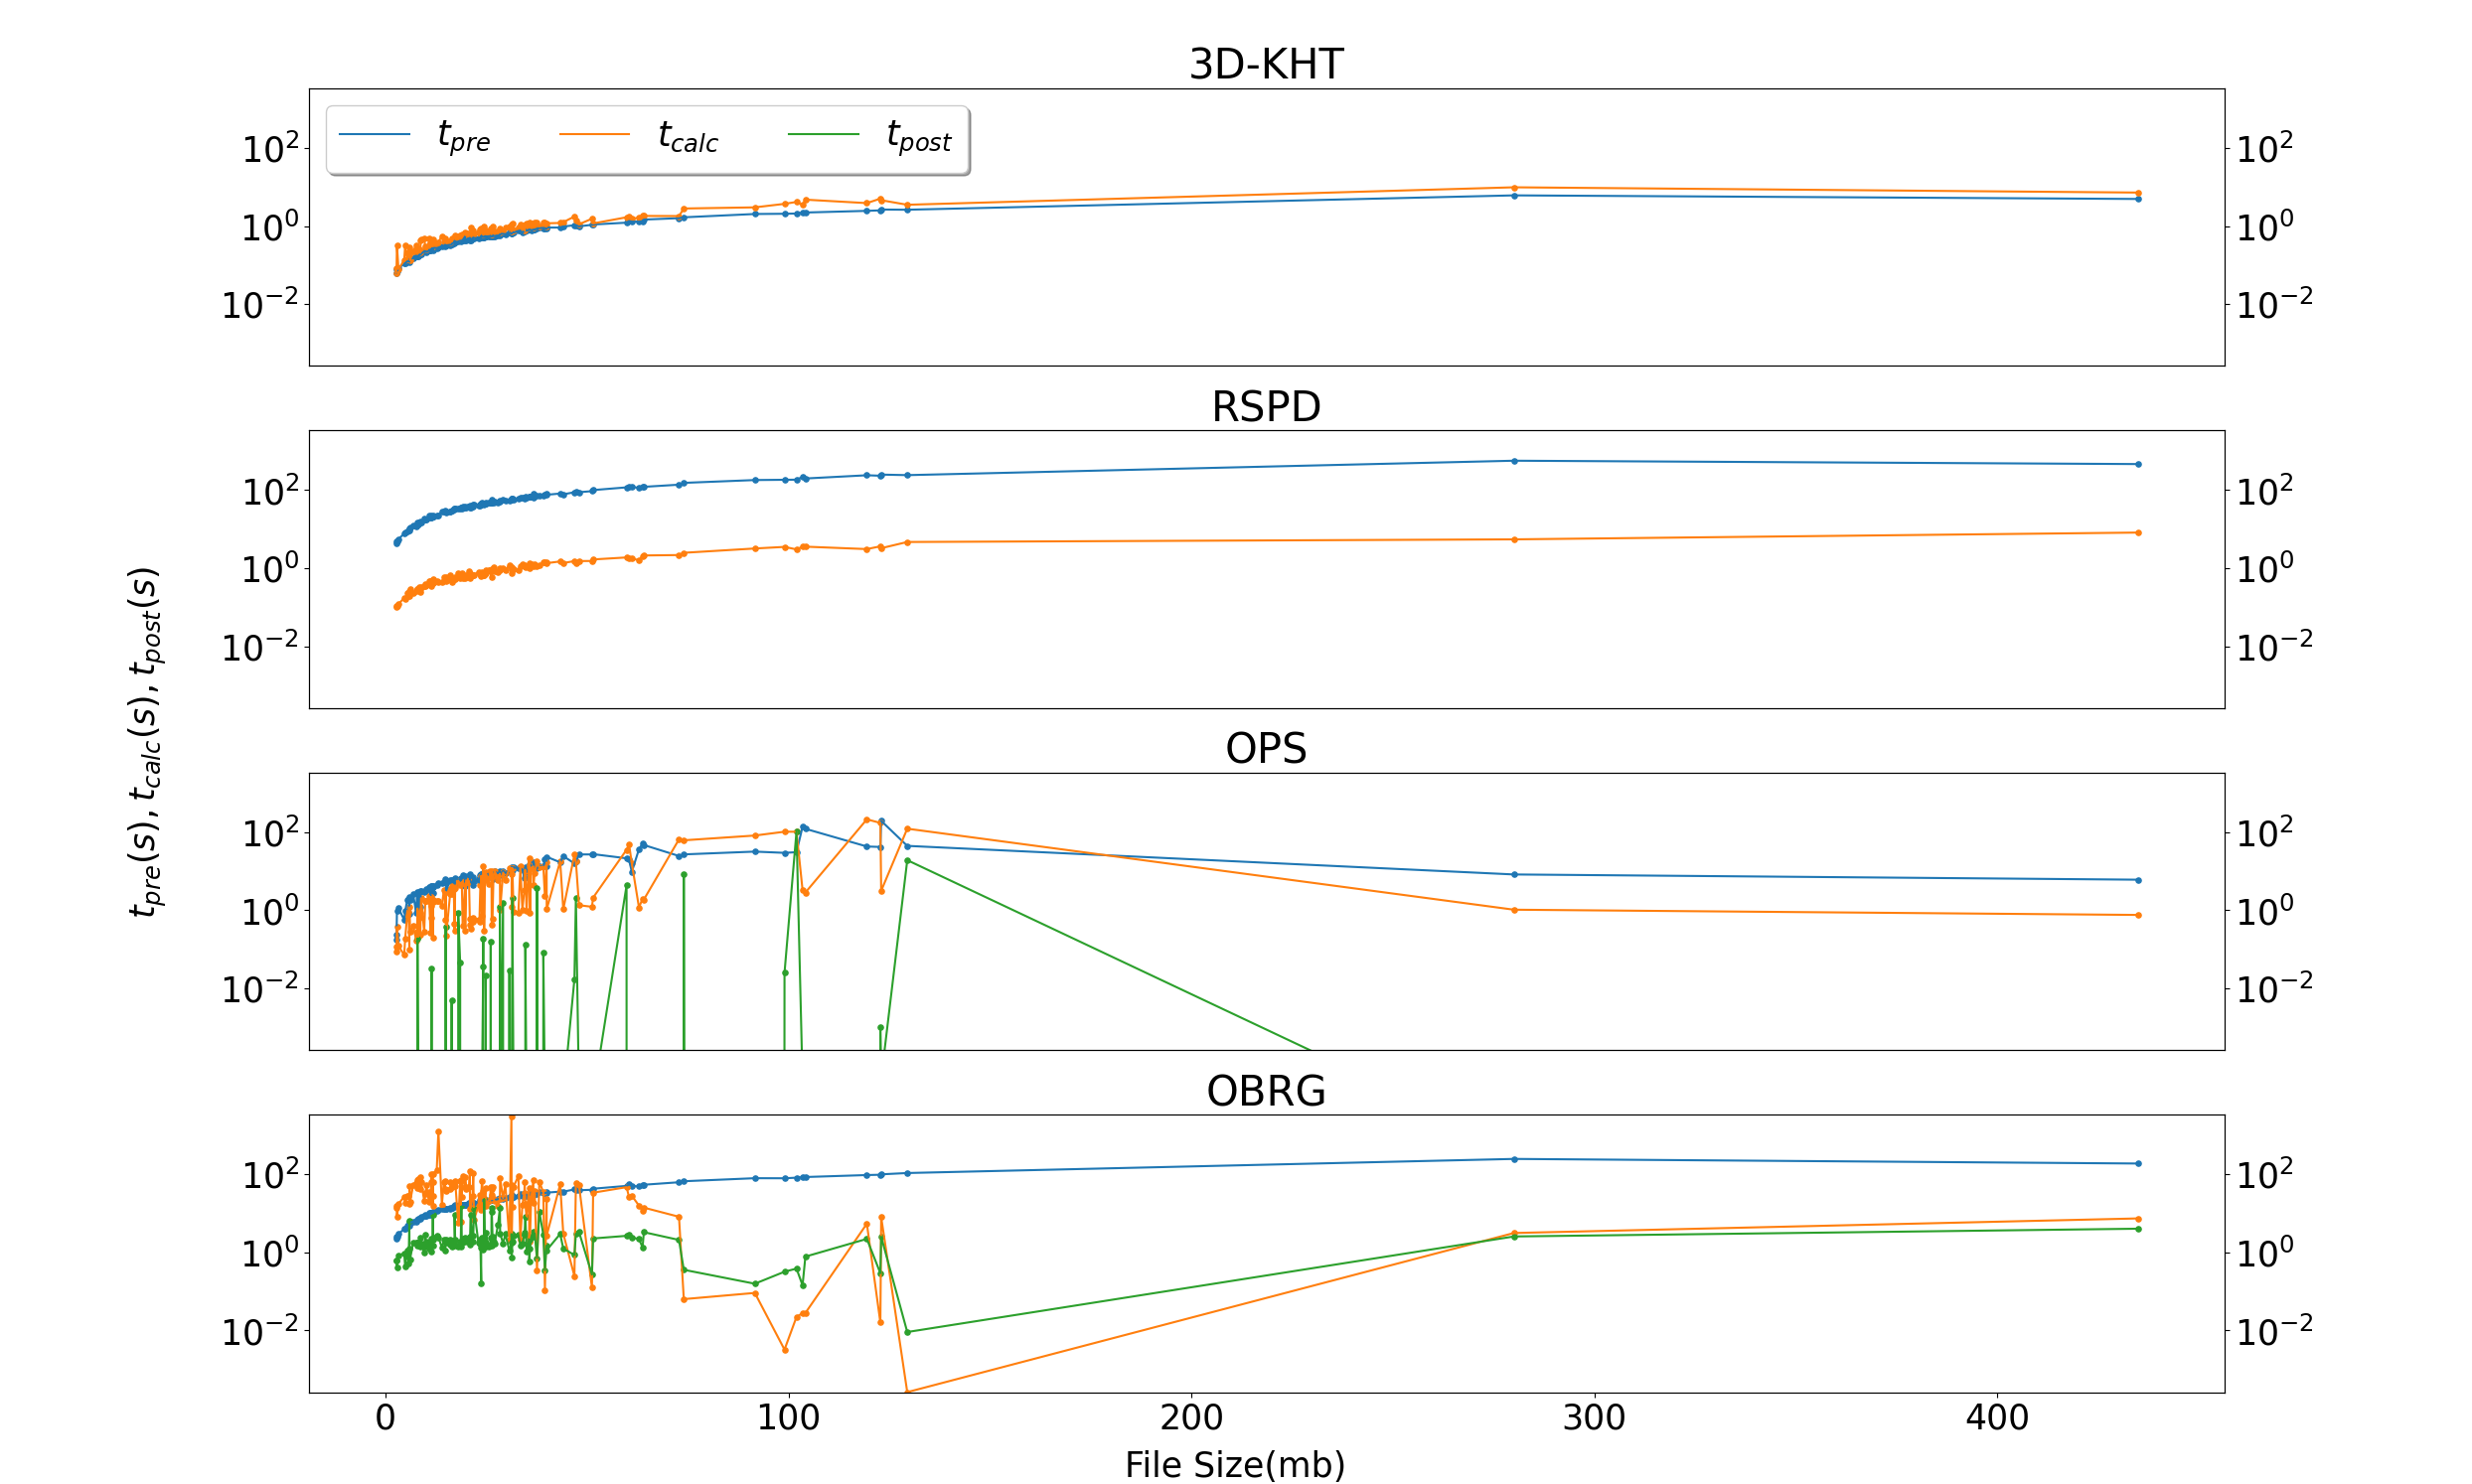
\includegraphics[width=\textwidth]{images/SDsizetime.png}
    \caption[Time per Cloud size 2D-3D-S]{Time spent in pre-processing ($t_{pre}$), plane detection ($t_{calc}$),
        and post-processing ($t_{post}$) per point cloud file size of the 2D-3D-S dataset. Note, that the y-axis is
        scaled logarithmically to the base of ten.}
    \label{fig:sizetimestanford}
\end{figure}
The computation times of 3D-KHT do not seem to strongly relate to the size of the point cloud.
Both the duration of the pre-processing and the duration of the plane detection initially grow linearly
but do not show a large growth even with large jumps in point cloud size.
The difference in calculation times between $100mb$ and ${>}200mb$ is hardly noticeable.

The computation times of RPSD show a similar relation, with the difference that the pre-processing of RSPD takes significantly longer.
As with 3D-KHT, the duration of plane detection seems to have an upper limit.

In general, the pre-processing time of OPS has a linear growth depending on the size of the point cloud.
The duration of plane detection also shows a linear relationship, with the difference that there is a certain level
of fluctuation. The post-processing times are negligible for the most part, given the values below $10^0$.
The irregularity of the spikes gives reason to assume that it primarily depends on the structure of the recorded
environment rather than size alone.

The duration of the pre-processing of OBRG also shows a linear relationship with respect to the point cloud size.
The average high $t_{pre}$ values from Table~\ref{tab:res-3d2ds-total} are also reflected here since most values are above ${\sim}10^1$.
The $t_{calc}$ values of OBRG do not appear to be dependent on the size of the point cloud, as the computation
times tend to decrease with growing point clouds. A possible reason could be the fixed value of the octree levels $l_{max}$.
An adaptive determination of octree size would likely lead to a more balanced curve.
Since the post-processing phase operates on the plane detection phase data, the curve behaves similarly,
supporting the sub-optimal parameterization argument.



\paragraph{Summary 2D-3D-S Experiment}
OPS has the highest value in Precision, while RSPD achieves the highest Accuracy and F1 score.
3D-KHT has the lowest total computation time $t_{tot}$ with an average of $1.74s$. With ${>}60s$,
RSPD and OBRG have the largest $t_{tot}$ values among the algorithms, with $t_{pre}$ accounting for
the majority for RSPD.

Figure~\ref{fig:sizetimestanford} shows that the runtimes of 3D-KHT are the smallest. RSPD also has low $t_{calc}$ values
but consistently spends the longest time in pre-processing.
Moreover, the pre-processing times of all algorithms seem to be generally dependent on the size of the point cloud.
The plane detection runtimes of OPS and OBRG fluctuate. However, OPS fluctuates less than OBRG.
The post-processing runtimes of OPS are negligible overall. The $t_{post}$ values of OBRG are stable at $2.61s$ on average,
except for medium cloud sizes, see table~\ref{tab:res-3d2ds-total}.

\subsection{FIN}
Each of the total 708 time frames of the FIN data set was processed by each algorithm.
Subsequently, we evaluated each time frame separately, i.e., by calculating the precision, the recall, and the F1 score.
Additionally, we measured the computation times of each time frame for all algorithms.

The average results over all time steps of all scenes of the FIN experiment are presented in Table~\ref{tab:res-fin-total}.
The highest values are written in bold for precision, recall, and the f1-score, as are the lowest times of each calculation step.


\begin{table}[H]
    \centering
    \begin{tabular}{c|cccccc|c}
        Algorithm & Precision        & Recall           & F1-Score         & $t_{pre}$     & $t_{calc}$    & $t_{post}$ & $t_{tot}$     \\ \hline
        RSPD      & 57.30\%          & \textbf{60.75\%} & \textbf{58.70\%} & 14.36         & \textbf{0.19} & /          & 14.55         \\
        OPS       & \textbf{69.38\%} & 29.23\%          & 39.43\%          & 4.61          & 0.89          & 0.13       & 5.63          \\
        3DKHT     & 49.76\%          & 44.40\%          & 46.48\%          & \textbf{0.14} & 0.29          & /          & \textbf{0.43} \\
        OBRG      & 49.23\%          & 27.42\%          & 33.94\%          & 6.03          & 14.70         & 0.35       & 21.08
    \end{tabular}
    \caption[Average FIN Results]{Average Results of the FIN experiment. Shown are the average values of all scenes and time frames, sorted by
        algorithm. The right half of the columns shows the average time spent in pre-processing ($t_{pre}$), the average time spent in the plane
        detection itself ($t_{calc}$), and the average time spent in post-processing steps ($t_{post}$).
        The rightmost column shows the average total calculation time $s_{tot}$.
        Note, that the absence of post-processing steps is denoted as "/".
        All times are measured in seconds.}
    \label{tab:res-fin-total}
\end{table}

\paragraph{Accuracy}
OPS has the highest average precision of the algorithms, with almost 70\%. RSPD, on the other hand, achieved the highest values
for recall and the F1-score. 3D-KHT and OBRG achieved a similar precision, but for Recall and F1 score, however, 3D-KHT has
higher values than OBRG by approx. 13\% and approx. 17\%, respectively. RSPD thus achieves the highest overall accuracy,
while OBRG achieves the overall lowest.


\paragraph{Average Time}
RSPD needs the most time in pre-processing among the algorithms. In contrast, RSPD has the shortest time spent
during plane detection, with 0.19 seconds. Overall, 3D-KHT needs the shortest time for the complete computation $t_{tot}$
of a time step with an average of $0.43$ seconds. OPS achieves comparatively average times with about 6 seconds, and OBRG
takes the longest overall to compute a time step with more than 20 seconds.


\paragraph{Relationship of Time and Size}

We want to consider the relationship between the size of the point cloud and the corresponding calculation time.
In Figure~\ref{fig:dynaudi}, we compare the processing times of each time step to the file size of the
\textit{auditorium} scene of the FIN data set.

Note, that we created similar graphs for the other scenes of the FIN dataset.
However, they do not introduce any new information in argumentation and are presented in the appendix \textbf{\textcolor{red}{\$REF}} for completeness
and spatial reasons.
The auditorium scene was selected because it represents the longest recording, and thus contains the most data.

\begin{figure}[H]
    \centering
    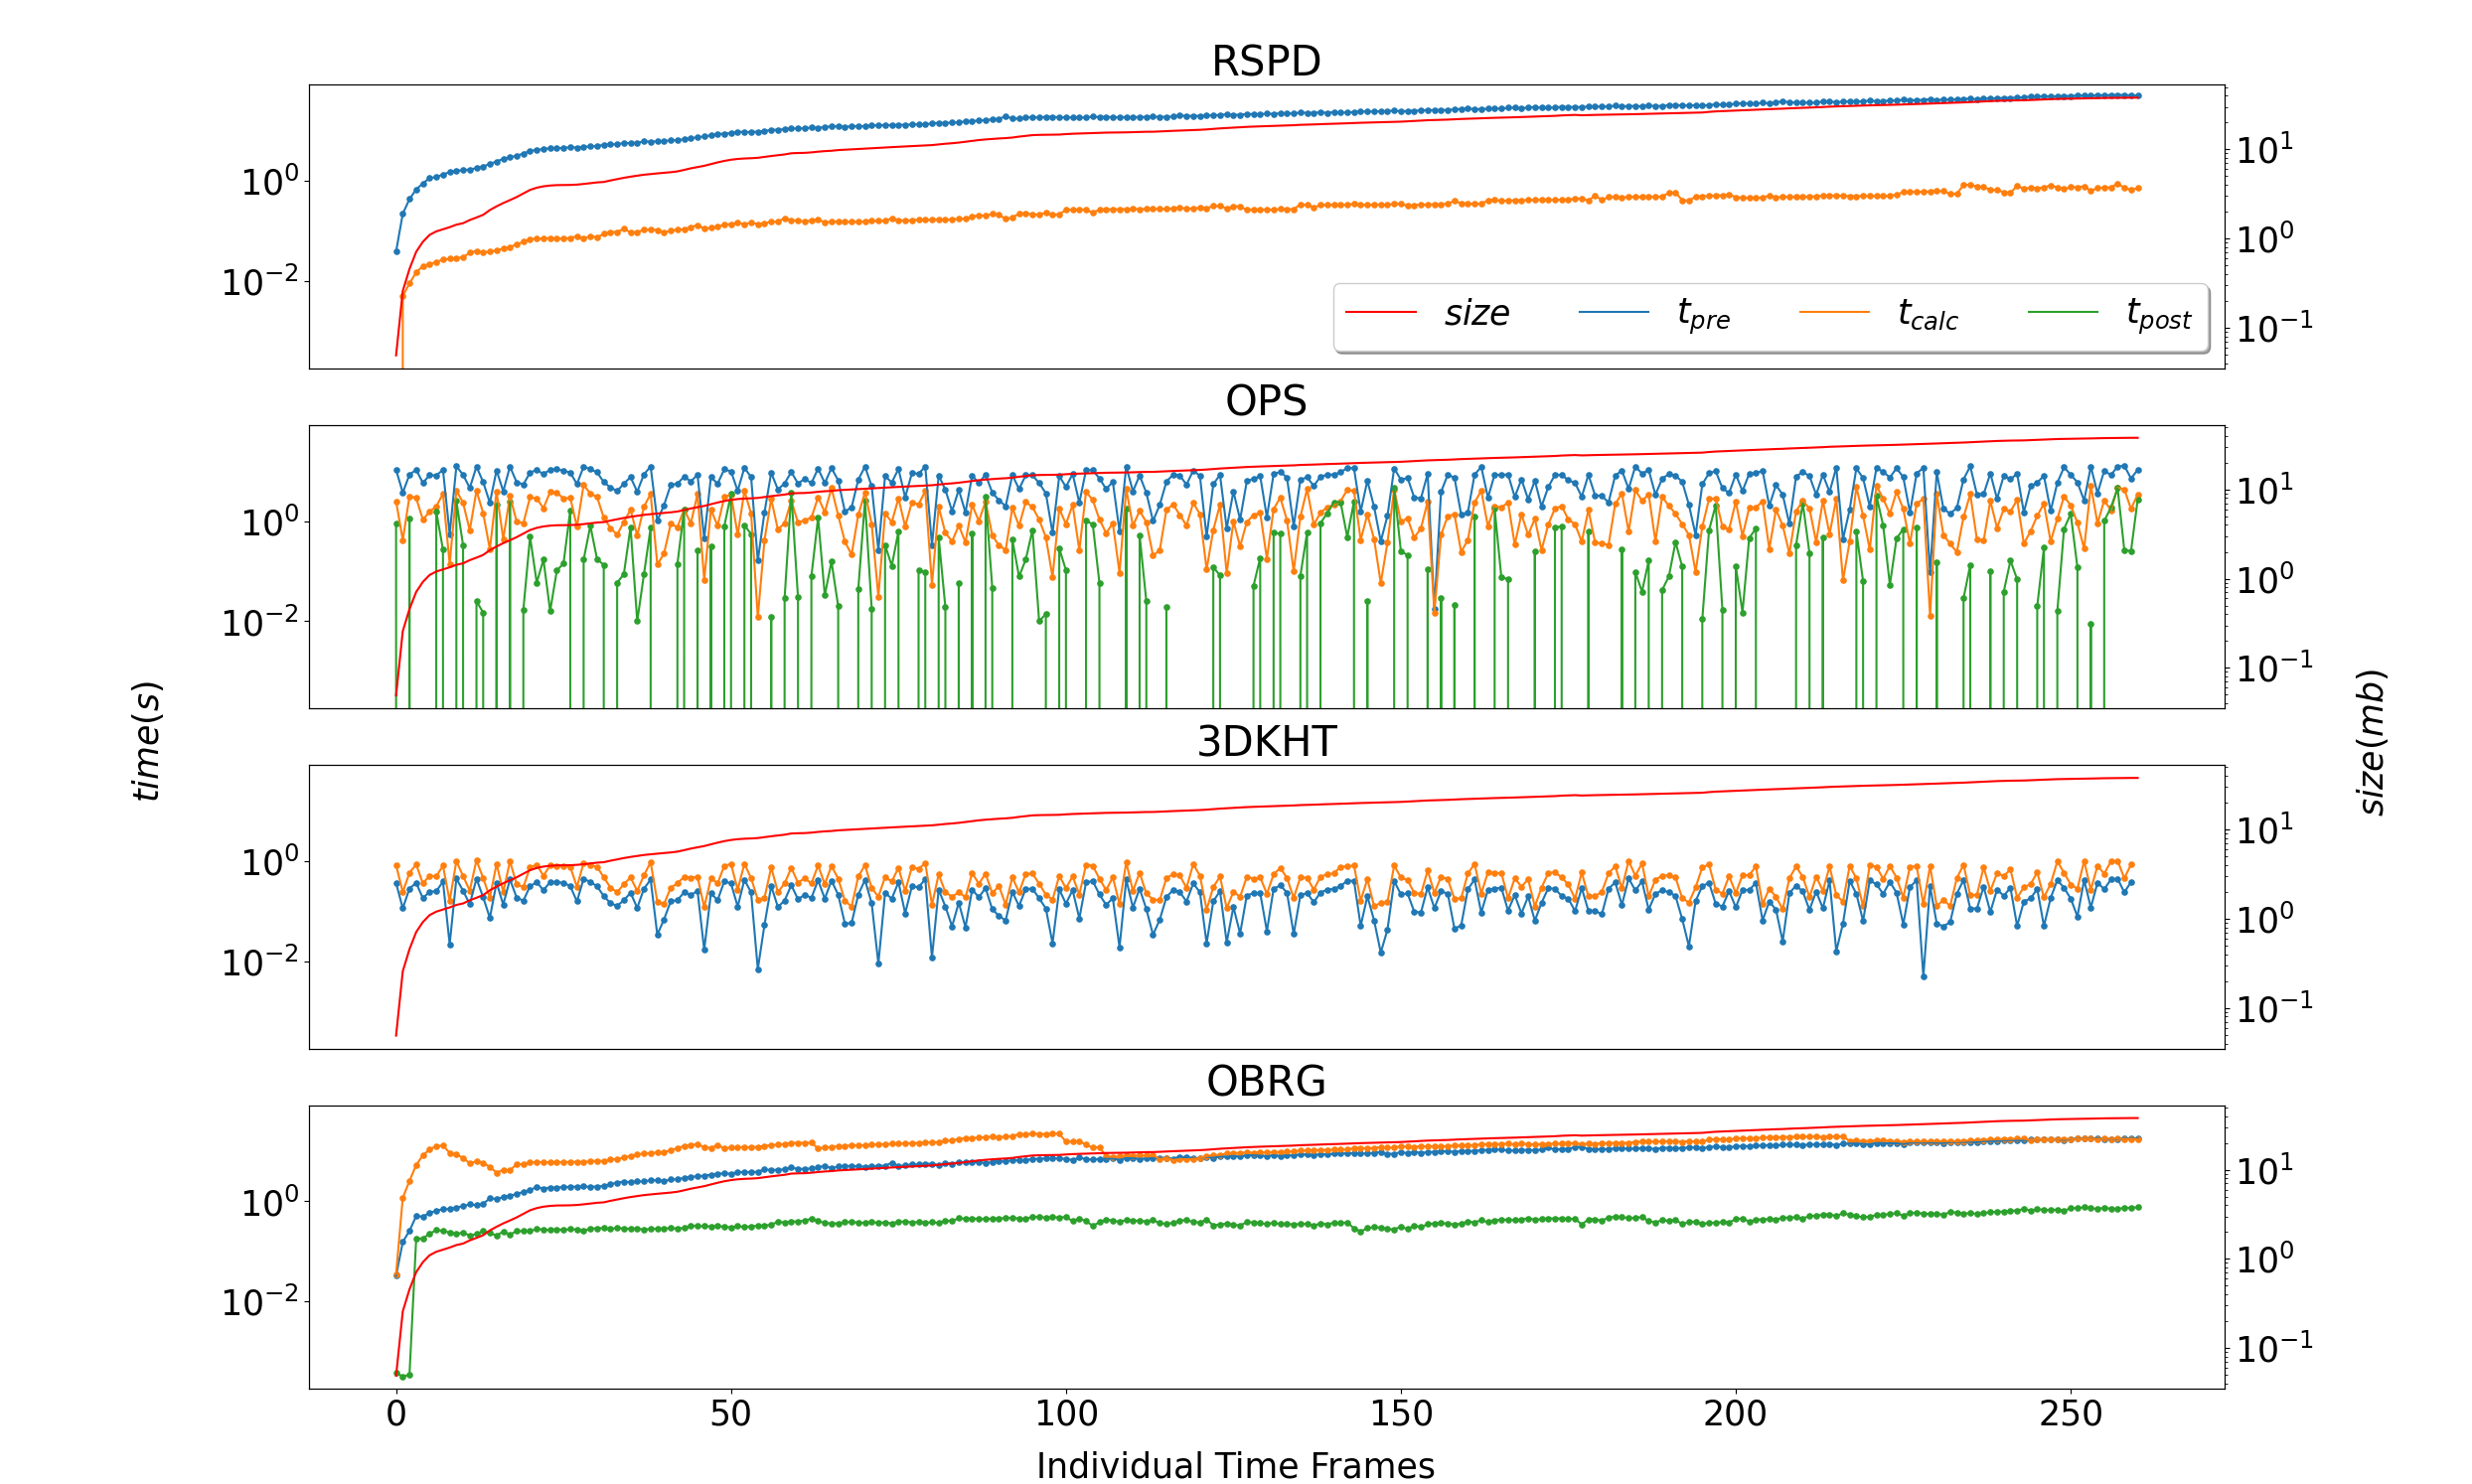
\includegraphics[width=\textwidth]{images/dyn_time-audi.png}
    \caption[Time Results Hallway]{Time spent in pre-processing (blue), plane detection (yellow), and post-processing
        (green) of the hallway scene and cloud sizes (red) of each time step. Note, that both y-axes are scaled
        logarithmically to the base of ten}
    \label{fig:dynaudi}
\end{figure}

The pre-processing times of RSPD and OBRG are noticeably proportional to the point cloud size.
In contrast, for OPS and 3D-KHT, the pre-processing times seem to correlate with the plane detection times since
both show similar spikes. The plane detection steps of OPS and 3D-KHT do not seem to depend on the point cloud size,
as both seem to be limited by an upper bound. The pre-processing and plane detection times of OBRG grow rapidly in the
beginning but afterward, show a linear growth in relation to the cloud size. The post-processing times of OPS fluctuate
between 0 and the duration of plane detection. After the spike in the beginning, the $t_{post}$ values of OBRG seem to be
consistent.

\paragraph{Summary FIN Experiment}
OPS has the highest average precision, and RSPD has the largest percentages in recall and F1 score. Additionally, RSPD has the lowest $t_{calc}$ value among the algorithms,
with an average of $0.19s$ per time frame. In contrast, RSPD has the longest pre-processing time with $14.36s$ on average.
The algorithm with the shortest pre-processing and the shortest total time is 3D-KHT with $t_{pre}=0.14$ and $t_{sum}=0.43$,
respectively.


In general, the calculation times of RSPD and OBRG seem to depend on the point cloud size.
However, the time RPSD spends in pre-processing is significantly higher than in its plane detection step.
In contrast, the pre-processing and plane detection times of OBRG seem to converge at the end.
The calculation times of OPS and 3D-KHT seem to be independent of the point cloud size and consistently stay under an upper bound.
However, 3D-KHT has a smaller upper bound than OPS.


\subsection{Comparison}
When comparing Table~\ref{tab:res-3d2ds-total} and Table~\ref{tab:res-fin-total}, a pattern emerges:
OPS has the highest precision value, RSPD yields the highest Recall and F1-Score, and 3D-KHT has the lowest
average total processing time.

Observing Figure~\ref{fig:dynaudi} and Figure~\ref{fig:sizetimestanford}, common features are noticeable:

The curve shape of RSPD is very similar for both experiments, linearly dependent on the point cloud size, and the
$t_{pre}$ accounts for $99\%$ of the total calculation time $t_{tot}$.
In both experiments, the post-processing time of OPS fluctuates.
The post-processing of OBRG seems to be mostly stable around a small value (${\sim}10^{-1}$).
3D-KHT scores very low processing times in both experiments.

However, there are also notable differences.
Whereas the calculation times of 3D-KHT seem to be proportional to the point cloud size in the 2D-3D-S experiment, they show no such
relation during the FIN experiment. It is, however, noteworthy that the cloud sizes widely differ between the experiments, as the
maximum size of the FIN experiment (${\sim}30mb$) is very small, compared to largest scene of the 2D-3D-S dataset (${>}400mb$).
Nonetheless, since Figure~\ref{fig:sizetimestanford} portrays a proportionality, even for smaller clouds, the reason for
different curves is likely the difference of parameterization.

\section{Summary}
OBRG does not achieve the highest or lowest values in any experiment.
OPS has the highest precision value in both experiments.
Due to Recall and the F1-score, RSPD has the highest overall accuracy in both experiments.
The pre-processing of RSPD takes the longest time of all algorithms. In contrast, RSPD has the smallest average $t_{calc}$
value in the FIN experiment. 3D-KHT has the lowest total computation time in both experiments, and in the 2D-3D-S experiment,
it outperforms the plane detection time of RSPD.


% NOTE 3DKHT kann keine löcher oder non-rectangular ebenen basteln!


\end{document}